\PassOptionsToPackage{subsection=false}{beamerouterthememiniframes}
\documentclass[a4,xcolor=dvipsnames]{beamer}

\mode<presentation> {
\usetheme{Berlin}
}

\definecolor{newBlue}{HTML}{2d4457} % 2d4457 UBC Blue (primary)

\usecolortheme[named=newBlue]{structure}

\usepackage[utf8]{inputenc}
\usepackage{amsmath}
\usepackage{amsthm}
\usepackage{amssymb}
\usepackage{algorithm}
\usepackage{tikz}
\usepackage{tikz-3dplot}
\usepackage{mathtools}
\usepackage[mathscr]{euscript}
\usepackage{algpseudocode}
\usepackage{epsfig}
\usepackage{adjustbox}
\usepackage{graphicx}
\usepackage{rotating}
\usepackage{booktabs}
\usepackage{multirow}
\usepackage{subcaption}
\usepackage{multicol}
\usepackage{float}
\usepackage{hyperref}
\usepackage{wrapfig}
\usetikzlibrary{shapes.geometric, arrows.meta}

\usetikzlibrary{positioning}
\usetikzlibrary{shapes,arrows}


\def\R{\mathbb{R}}

\def\a{\mathbf{a}}
\def\b{\mathbf{b}}
\def\x{\mathbf{x}}
\def\y{\mathbf{y}}
\DeclareMathOperator*{\argmin}{argmin}
\DeclareMathOperator*{\argmax}{argmax}


\newcommand\blfootnote[1]{%
  \begingroup
  \renewcommand\thefootnote{}\footnote{#1}%
  \endgroup
}

\makeatletter
\def\blfootnote{\gdef\@thefnmark{}\@footnotetext}
\makeatother

\AtBeginSection[]{
  \begin{frame}
  \vfill
  \centering
  \begin{beamercolorbox}[sep=8pt,center,shadow=true,rounded=true]{title}
    \usebeamerfont{title}\secname\par%
  \end{beamercolorbox}
  \vfill
  \end{frame}
}


\pgfdeclarelayer{bg}    % declare background layer
\pgfsetlayers{bg,main}

\title{Machine Learning for Signal Processing: Lecture 2}
\author{Seyyid Emre Sofuo\u{g}lu}

\begin{document}

\setlength{\leftmargini}{0.2cm}

\begin{frame}
    \maketitle
\end{frame}
\begin{frame}
    \frametitle{Regression}
    $\mathbf{x} \in \mathbb{R}^N$, $\y\in \{-1,1\}^M$,
    \begin{gather*}
        A\mathbf{x}+\mathbf{b} = \mathbf{y},
    \end{gather*}
    variables $A\in\mathbb{R}^{M\times N}$, $\b\in\R^{M}$.
    \begin{itemize}
        \item Least squares: $(y-(ax+b))^2 \rightarrow \|\y-A\x-\b\|_2^2$.
        \item $X = [\x_1, \x_2, \x_3,\dots, \x_K]$, $Y = [\y_1, \y_2, \dots, \y_K]$ 
        \begin{align*}
            Y &= AX + \b \\
            Y &= [A, \b] [X^\top, \mathbf{1}]^\top = \hat{A} \hat{X} \\
            \hat{A} & = Y \hat{X}^{-1} \\
            \hat{A} &= Y(\hat{X}^\top\hat{X})^{-1}\hat{X}^\top 
        \end{align*}
    \end{itemize}
\end{frame}

\begin{frame}
    \frametitle{Support Vector Machines}
\begin{itemize}
    \item Searches largest margin between classes.
\end{itemize}
\begin{gather*}
    \min_{\a} \|\a\|^2, \quad \text{s.t.} y_i(\a^\top\x_i+b)\geq 1, \forall i
\end{gather*}
\begin{figure}[H]
    \centering
    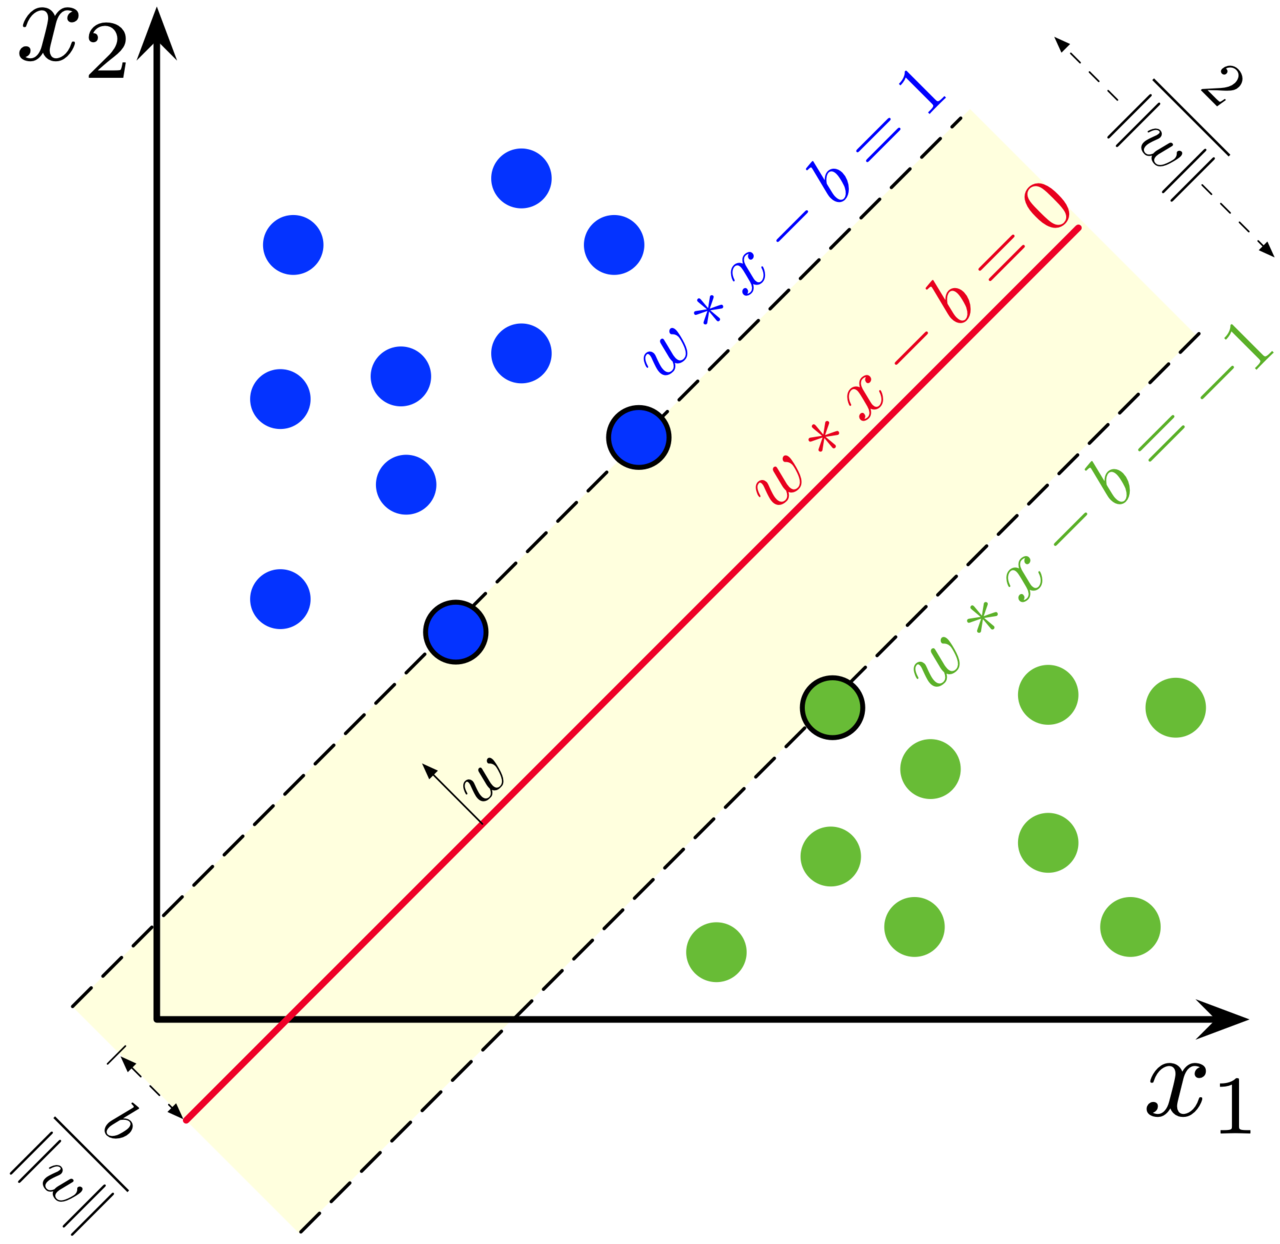
\includegraphics[width=.5\textwidth]{SVM_margin.png}
\end{figure}
\begin{itemize}
    \item "Supported" by vectors: SVM. No idea about "Machine"
    \item Hard vs soft margins
\end{itemize}
\begin{gather*}
    \min_{\a} \lambda\|\a\|^2+\frac{1}{N}\sum_{i=1}^N \max(0, 1-y_i(\a^\top\x_i+b))
\end{gather*}
\end{frame}

\begin{frame}
    \frametitle{Neural Networks: Multi-Layer Perceptron}
\begin{itemize}
    \item Regression+Activation
\end{itemize}

\begin{minipage}{.49\textwidth} 
    \begin{figure}[H]
        \centering
        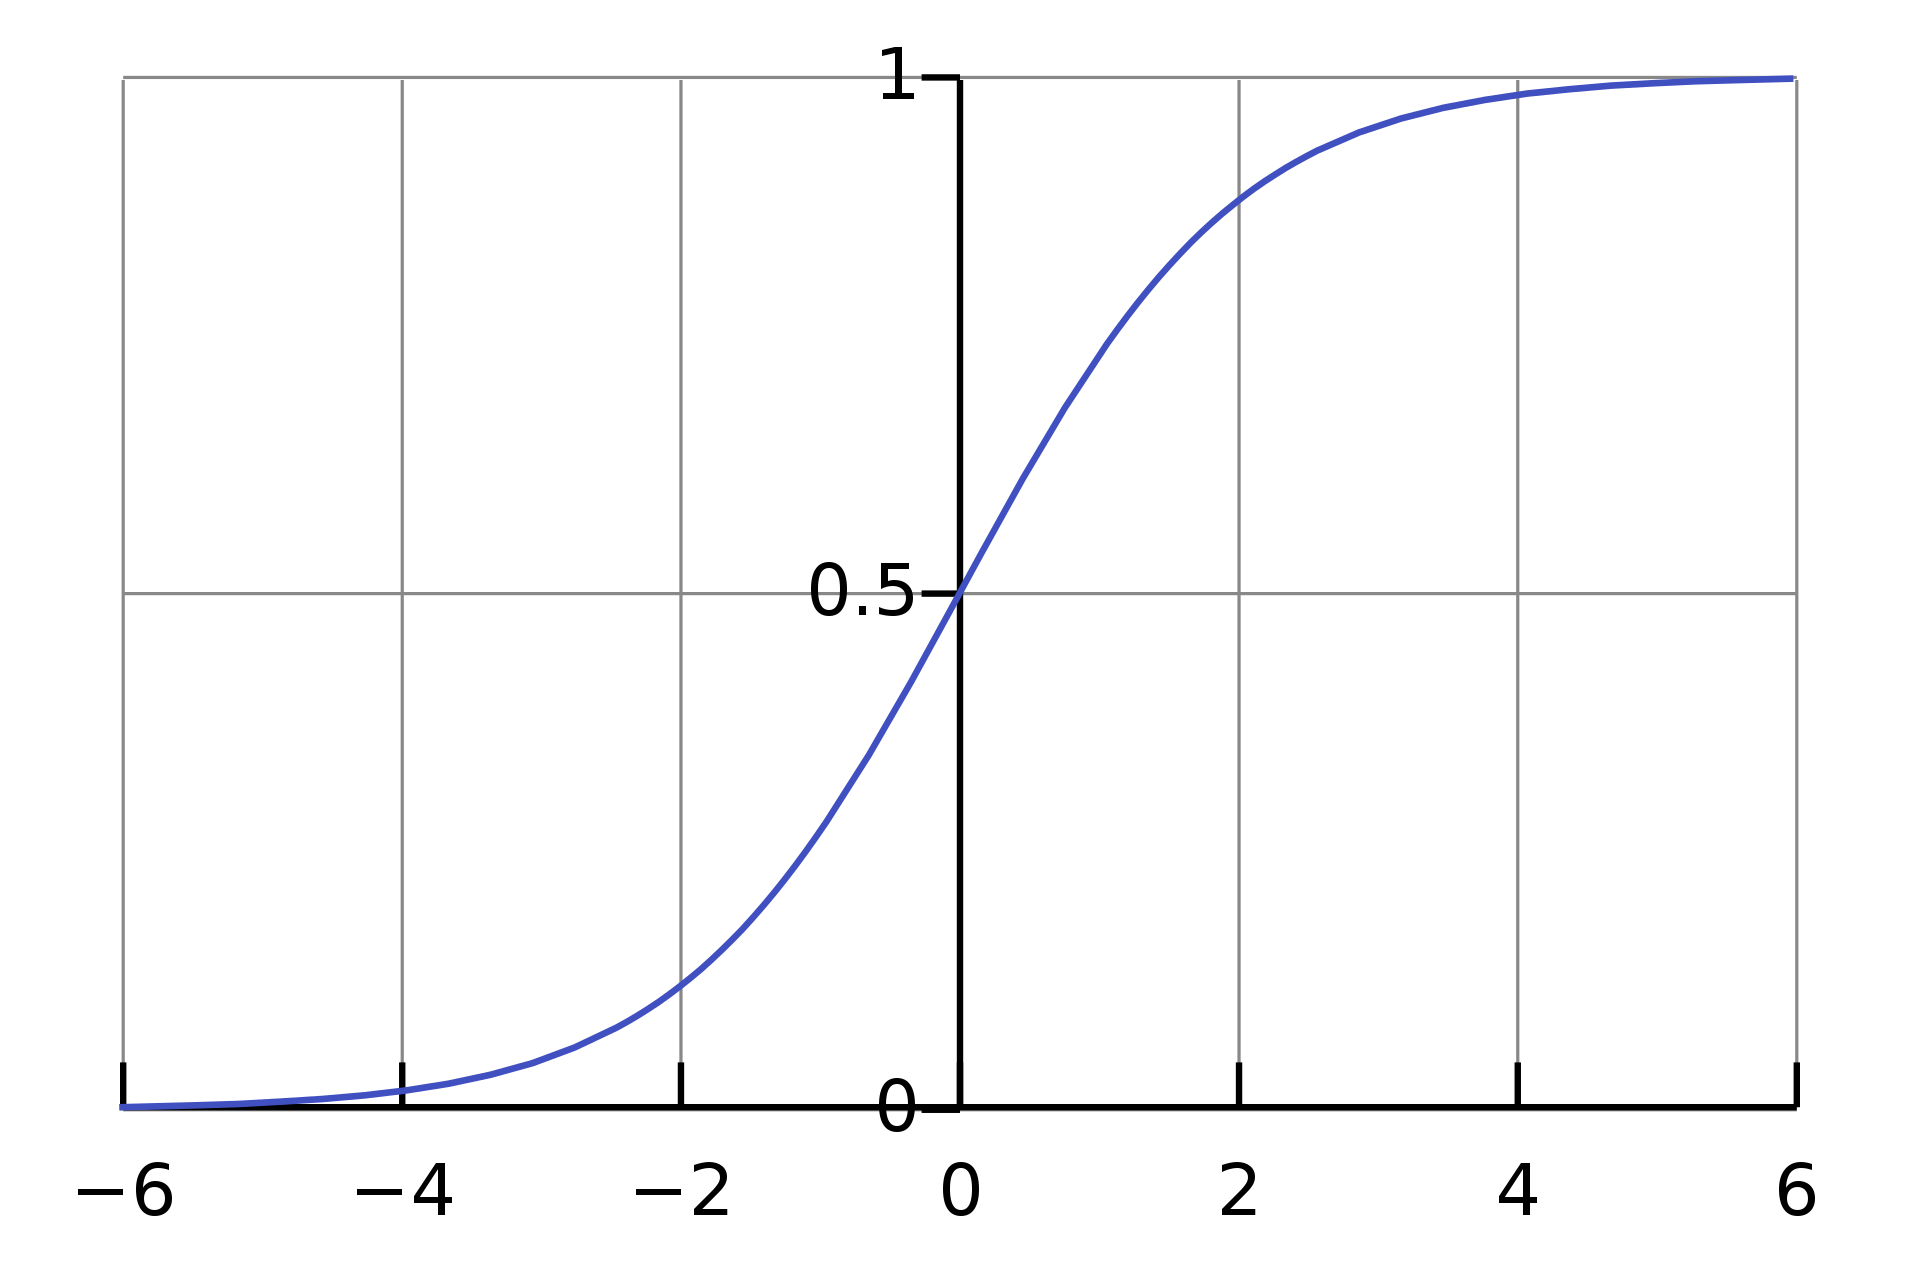
\includegraphics[width=.5\textwidth]{activation.png}
    \end{figure}
\end{minipage}
\begin{minipage}{.49\textwidth}
    \tikzset{
        net node/.style = {circle, minimum width=1.5 em, inner sep=0pt, outer sep=0pt, outer color=green!25!gray!50!cyan, inner color=green!25!gray!50!cyan},
        net2 node/.style = {circle, minimum width=1.5 em, inner sep=0pt, outer sep=0pt, outer color=blue!25!gray!50!cyan, inner color=blue!25!gray!50!cyan},
        net3 node/.style = {circle, minimum width=1.5 em, inner sep=0pt, outer sep=0pt, outer color=red!25!gray, inner color=red!25!gray}
        }
    \begin{figure}[H]
        \centering
        \adjustbox{width=.7\columnwidth}{
        \begin{tikzpicture}
            \foreach \i in {1,...,4}{
                \draw (0, \i*1+0.5) node (l1\i) [net node] {};
                }
            \foreach \i in {1,...,5}{
                \draw (2, \i*1) node (l2\i) [net2 node] {};}
            \foreach \i in {1,...,3}{
                \draw (4, \i*1+1) node (l3\i) [net3 node] {};}
            \foreach \i in {1,...,5}{
                \foreach \j in {1,...,4}{
                    \draw (l1\j) -- (l2\i);}
                \foreach \j in {1,...,3}{
                    \draw (l2\i) -- (l3\j);}
            }
            \draw (1, 6) node {$A_1\in\R^{4\times5}$};
            \draw (3, 6) node {$A_2\in\R^{5\times3}$};
            \draw (0, 0.5) node {\footnotesize Input Layer};
            \draw (2, 0) node {\footnotesize Hidden Layer};
            \draw (4, 1) node {\footnotesize Output Layer};
        \end{tikzpicture}}
    \end{figure}
\end{minipage}
\begin{itemize}
    \item Without activation, stacking MLPs is meaningless.
    \item With activation, every layer has inputs and outputs $\rightarrow$ every layer can be trained.
\end{itemize}
\end{frame}

\begin{frame}
    \frametitle{Neural Networks, continued}
    \begin{figure}
        \centering
        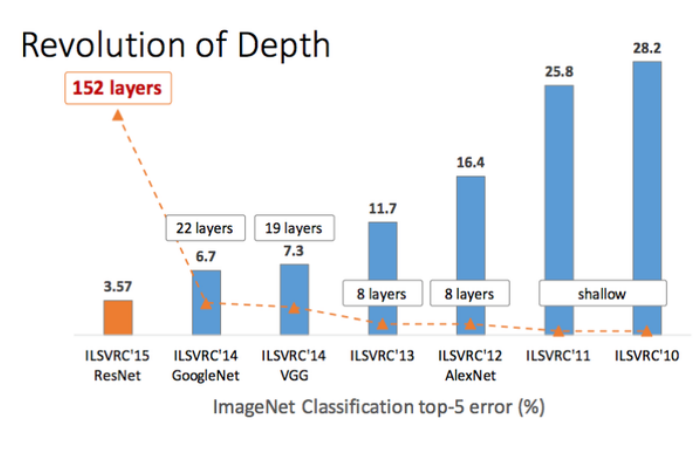
\includegraphics[width=.7\textwidth]{depth.png}
    \end{figure}
\end{frame}

\end{document}